\section{Rehearsals on the Real Simulator}
\label{sec:results}
Each rehearsal is a complete 20-call, 1,000-point run of a policy on a local copy of the released simulator
(sha256-pinned), with the policy's own pre-submit screen and log. Table~\ref{tab:online} lists the best $R$ of every
run; Fig.~\ref{fig:convergence} shows the best value per call.

\begin{table}[t]
\centering
\caption{Best $R$ (kWh) after 20 calls $\times$ 50 points on the real simulator, by policy and seed. Best offline
result: 115.68; best training row: 115.76.}
\label{tab:online}
\setlength{\tabcolsep}{4pt}
\begin{tabular}{lrrrr}
\toprule
Policy & seed 2026 & seed 7 & seed 11 & mean\\
\midrule
v1: block descent & 107.03 & 107.21 & 106.43 & 106.89\\
v2: v1 + training shift bias & 106.95 & 105.11 & 107.49 & 106.52\\
v4: v2 + evidence-driven slots & 108.05 & 103.28 & 105.44 & 105.59\\
v5: v4 + vertex probes, lanes & 106.17 & 106.18 & 106.44 & 106.26\\
v6: v4 + lanes when stalled & 107.41 & 106.48 & 106.68 & 106.86\\
v4, fixed-constant GP & 106.43 & 105.08 & 107.15 & 106.22\\
\textbf{h7: v4 + hybrid (submitted)} & 107.81 & \textbf{102.81} & 105.87 & 105.50\\
\bottomrule
\end{tabular}
\end{table}

\begin{figure}[t]
\centering
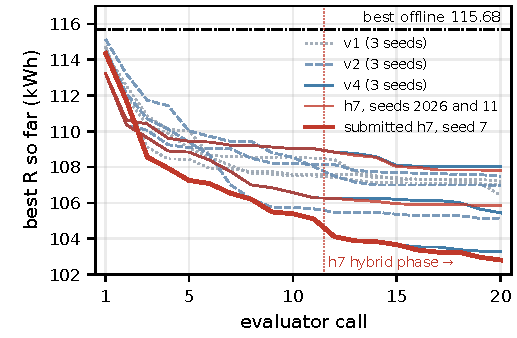
\includegraphics[width=\columnwidth]{figures/convergence.pdf}
\caption{Best measured $R$ per call. Thin lines: v1, v2 and v4, three seeds each; red: the submitted h7 (thick: seed 7,
the submitted seed; thin: seeds 2026 and 11), identical to v4 with the same seed up to call 11. Source: logs in
\texttt{analysis/online\_rehearsal/}, \texttt{analysis/online\_v7/} and \texttt{analysis/online\_v7\_seeds/} (real
simulator, no surrogate values).}
\label{fig:convergence}
\end{figure}

\textbf{Every run beats the offline result in the first call.} All 16 runs of v1--v6 send a first batch whose minimum
lies between 113.2 and 115.1, below our offline 115.68, using only the training rows. Most of the descent happens in
calls 1--5 (to 107--110), after which gains shrink to tenths of a kWh per call.

\textbf{Seeds matter as much as variants.} Variant means lie within 105.6--106.9 while the seeds of one variant span
up to 4.8~kWh (v4: 103.28--108.05), so with three seeds no variant is established as better than v4. Two attempts to
avoid early commitment to one ``form'' per building (v5, v6) and a surrogate with fixed hyperparameters did not help.
The move statistics explain why v4 kept its place: over three seeds, the share of points that beat their call's base was
3.0\,\% for model picks, 7.6\,\% for random moves, 8.8\,\% for fine moves and 7.7\,\% for scans, and scans produced most late
gains. Combinations confirmed additivity online: measured minus predicted had median $+0.013$ and MAE 0.22 over 214
points, whereas the surrogate's own picks landed on average 3.6 above their prediction.

\textbf{The submitted policy.} h7 with seed 7 reaches 102.81 (Fig.~\ref{fig:batches}), 0.47 below v4 with the same seed;
the two runs are identical up to call 15 and diverge from call 16, and the single largest new contribution is one coarse
move at call 19 ($-0.28$). Because h7 was designed on that seed's log, we then ran the graded package unchanged on
seeds 2026 and 11. In calls 1--11 it sends the same batches as v4 and every point gets the same $R$ (apart from a
last-bit difference in four weight vectors and one swapped tie), so the comparison is paired. In calls 12--18 h7's best
value is at or below v4's on all three seeds; after call 20 it is 0.24 below v4 on seed 2026 and 0.43 above on seed 11,
where v4's last two calls dropped from 106.02 to 105.44. The paired mean difference is $-0.09$ ($-0.47$, $-0.24$,
$+0.43$), well inside the seed spread: h7 brings late gains forward but is not shown to end lower than v4.

\begin{figure}[t]
\centering
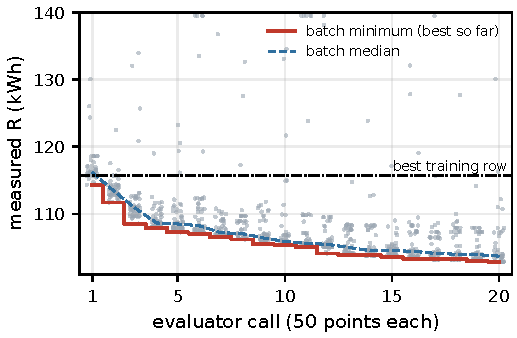
\includegraphics[width=\columnwidth]{figures/h7_batches.pdf}
\caption{All 1,000 measured points of the submitted run (h7, seed 7; values above 139.5 clipped). The score of a call is
its minimum; the batch median stays high because most slots probe, and only the minimum needs to be low.}
\label{fig:batches}
\end{figure}
